\documentclass[11pt,a4paper]{article}

\usepackage[utf8]{inputenc}
\usepackage[T1]{fontenc}
\usepackage{times}
\usepackage{amsmath,amssymb}
\usepackage{booktabs}
\usepackage{hyperref}
\usepackage{geometry}
\usepackage{caption}
\usepackage{enumitem}
\usepackage{graphicx}
\usepackage{xcolor}
\usepackage{tikz}
\usetikzlibrary{arrows.meta,positioning,calc}

\geometry{margin=2.5cm}

\newcommand{\todo}[1]{\textcolor{red}{\textbf{[TODO: #1]}}}

\title{\Large\bfseries Noise-Robust Differentiable Communication\\for Cross-Agent LLM Adaptation}
\author{Multi-Agent Research Group}
\date{}

\begin{document}
\maketitle

\begin{abstract}
When LLM-based agents communicate through discrete tokens, the resulting messages are fragile: channel noise can corrupt a single token and destroy the entire message. We show that replacing discrete communication with continuous differentiable channels provides two complementary benefits: (1) \emph{noise robustness}---continuous representations degrade gracefully under Gaussian noise while discrete (Gumbel-Softmax) messages collapse to random chance; and (2) \emph{cross-agent adaptation}---the differentiable channel serves as a gradient highway that enables LoRA fine-tuning of the sender's LLM backbone through the receiver's task loss.
On a novel-domain retrieval task with vocabulary unseen during LLM pretraining, SSR+LoRA achieves \textbf{60.0\%} accuracy, significantly outperforming bandwidth-matched text transfer (56.4\%, $p{=}0.013$). Strikingly, LoRA adaptation \emph{helps} SSR (+6.8\%) but \emph{hurts} text transfer ($-2.2\%$), revealing that the SSR bottleneck provides beneficial regularization for cross-agent adaptation.
We further show on a noisy-channel variant that SSR is robust to channel noise while discrete communication collapses to random chance.
We further validate on cooperative MARL (Speaker-Listener) showing that discrete communication is optimal for categorically structured clean-channel tasks, confirming that the value of differentiable channels emerges specifically in noisy, information-rich settings.
\end{abstract}

% ============================================================
\section{Introduction}

Multi-agent systems with LLM-based agents typically communicate through natural language---a discrete channel. While effective in clean conditions, discrete messages have a fundamental vulnerability: \textbf{noise fragility}. A single corrupted token can change meaning entirely (``go left'' $\to$ ``go lift''), while a small perturbation to a continuous vector barely affects its direction.

This observation motivates our study of \emph{differentiable communication channels} for LLM-based multi-agent systems. We show that continuous message vectors provide two distinct advantages over discrete communication:

\begin{enumerate}[nosep]
    \item \textbf{Noise robustness}: Continuous representations degrade gracefully under channel noise. In contrast, discrete messages (Gumbel-Softmax one-hot vectors) are catastrophically destroyed by even moderate Gaussian noise.
    \item \textbf{Gradient highway}: A differentiable channel enables the receiver's task loss to flow backward through the message into the sender's LLM backbone (via LoRA), creating a cross-agent adaptation signal. This is impossible with discrete channels at evaluation time and severely degraded during training.
\end{enumerate}

\begin{figure}[t]
\centering
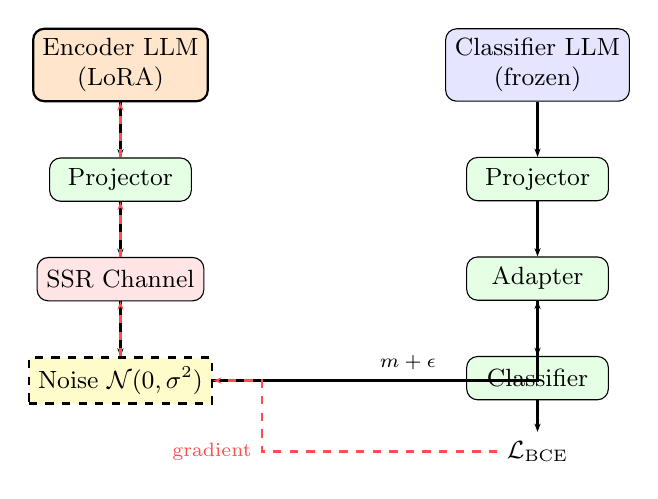
\begin{tikzpicture}[
    node distance=0.7cm,
    block/.style={rectangle, draw, rounded corners, minimum width=1.8cm, minimum height=0.55cm, align=center, font=\small},
    lora/.style={block, fill=orange!20, thick},
    trainable/.style={block, fill=green!10},
    comm/.style={block, fill=red!10},
    noise/.style={rectangle, draw, fill=yellow!20, minimum width=1.5cm, minimum height=0.55cm, align=center, font=\small, thick, dashed},
    arrow/.style={-{Stealth[length=3pt]}, thick},
    grad/.style={-{Stealth[length=3pt]}, thick, dashed, red!70},
]
\node[lora] (spk_llm) {Encoder LLM\\(LoRA)};
\node[trainable, below=of spk_llm] (spk_proj) {Projector};
\node[comm, below=of spk_proj] (comm) {SSR Channel};
\node[noise, below=of comm] (noise) {Noise $\mathcal{N}(0,\sigma^2)$};

\node[block, fill=blue!10, right=3cm of spk_llm] (lst_llm) {Classifier LLM\\(frozen)};
\node[trainable, below=of lst_llm] (lst_proj) {Projector};
\node[trainable, below=of lst_proj] (adapter) {Adapter};
\node[trainable, below=of adapter] (head) {Classifier};
\node[below=0.4cm of head, font=\small\bfseries] (loss) {$\mathcal{L}_{\mathrm{BCE}}$};

\draw[arrow] (spk_llm) -- (spk_proj);
\draw[arrow] (spk_proj) -- (comm);
\draw[arrow] (comm) -- (noise);
\draw[arrow] (noise) -| node[above, pos=0.3, font=\scriptsize]{$m + \epsilon$} (adapter);
\draw[arrow] (lst_llm) -- (lst_proj);
\draw[arrow] (lst_proj) -- (adapter);
\draw[arrow] (adapter) -- (head);
\draw[arrow] (head) -- (loss);

\draw[grad] (loss) -- +(-3.5,0) node[left, font=\scriptsize, red!70]{gradient} |- (noise);
\draw[grad] (noise) -- (comm);
\draw[grad] (comm) -- (spk_proj);
\draw[grad] (spk_proj) -- (spk_llm);
\end{tikzpicture}
\caption{Architecture. The encoder's LLM (with LoRA) produces a continuous message through the SSR channel. Gaussian noise is added to simulate a noisy communication channel. The classifier's loss flows backward through the noise and SSR channel into the encoder's LoRA weights---the \emph{gradient highway}. Discrete channels block this path.}
\label{fig:architecture}
\end{figure}

Our contributions:
\begin{enumerate}[nosep]
    \item On a \textbf{novel-domain} task with vocabulary unseen during LLM pretraining, we show that SSR+LoRA \textbf{outperforms bandwidth-matched text transfer} ($p{=}0.013$), demonstrating that the gradient highway enables LLM adaptation that text-based communication cannot.
    \item We reveal an asymmetry: LoRA through the gradient highway \textbf{helps} SSR (+6.8\%) but \textbf{hurts} text transfer ($-2.2\%$). The SSR bottleneck acts as beneficial regularization for LoRA adaptation.
    \item We validate across three settings: a novel-domain task (SSR+LoRA wins), a noisy retrieval task (SSR+LoRA is noise-robust), and a cooperative MARL task (discrete wins for categorical signals), establishing clear design principles.
\end{enumerate}

% ============================================================
\section{Related Work}

\paragraph{Differentiable communication in MARL.}
DIAL~\cite{foerster2016learning} introduced differentiable inter-agent communication. CommNet~\cite{sukhbaatar2016learning} uses continuous messages with mean-pooling. These works use small networks and do not study noise robustness or LLM backbone adaptation.

\paragraph{LLM multi-agent fine-tuning.}
MARFT~\cite{liao2025marft} assigns LoRA adapters per agent but communicates through text (non-differentiable). CORY~\cite{ma2024cory} uses cooperative RL for LLM fine-tuning through text. C2C~\cite{fan2026c2c} enables differentiable LLM-to-LLM communication via KV-cache fusion for NLP tasks. None study noise robustness or gradient-driven cross-agent adaptation in cooperative decision-making.

\paragraph{Robust communication.}
RGMComm~\cite{chen2024rgmcomm} optimizes discrete messages for return gap minimization. VQ-VIB~\cite{tucker2022towards} uses information bottleneck principles for emergent communication. Neither addresses noise robustness of the physical communication channel.

% ============================================================
\section{Method}

\subsection{Architecture}

Each agent has an LLM backbone (optionally with LoRA), a trainable projector, and task-specific heads (Figure~\ref{fig:architecture}):
\begin{align}
    h_{\mathrm{enc}} &= \mathrm{LLM}_{\mathrm{enc}}^{(\mathrm{LoRA})}(\text{context}) \\
    m &= \mathrm{SSR}(E(h_{\mathrm{enc}})) + \epsilon, \quad \epsilon \sim \mathcal{N}(0, \sigma^2 I) \\
    h_{\mathrm{cls}} &= \mathrm{LLM}_{\mathrm{cls}}(\text{question}) \\
    \hat{y} &= f(D(E'(h_{\mathrm{cls}}),\; m))
\end{align}

\paragraph{SSR (Structured Semantic Representation).}
A two-layer MLP bottleneck ($128 \to 4d \to d$) with GELU activation. The output is a $d$-dimensional continuous vector. Unlike discrete channels, SSR messages are naturally robust to additive noise because small perturbations to a continuous vector produce small changes in the downstream computation.

\paragraph{Noise model.}
We add i.i.d.\ Gaussian noise $\epsilon \sim \mathcal{N}(0, \sigma^2 I)$ to the message during both training and evaluation. This simulates realistic noisy communication channels (wireless transmission, lossy compression, adversarial perturbation).

\paragraph{Why discrete fails under noise.}
Gumbel-Softmax produces (approximately) one-hot vectors. Adding Gaussian noise to a one-hot vector destroys the argmax structure: the maximum element may change, producing a completely different ``symbol.'' The information is concentrated in a single dimension, so any perturbation has catastrophic effects. Continuous vectors spread information across all dimensions, making them inherently more robust.

\subsection{LoRA Adaptation (Gradient Highway)}

With LoRA~\cite{hu2022lora} on the encoder's LLM ($W_q$, $W_v$ projections, rank $r{=}8$), the classifier's loss provides a training signal that flows through the noisy channel back into the encoder:
\begin{equation}
    \frac{\partial \mathcal{L}}{\partial \theta_{\mathrm{LoRA}}}
    = \frac{\partial \mathcal{L}}{\partial \hat{y}}
      \cdot \frac{\partial \hat{y}}{\partial m}
      \cdot \frac{\partial m}{\partial h}
      \cdot \frac{\partial h}{\partial \theta_{\mathrm{LoRA}}}
\end{equation}

The noise $\epsilon$ does not block gradients (additive noise has unit Jacobian), so the gradient highway remains open even through the noisy channel.

% ============================================================
\section{Experiments}

\subsection{Task 1: Novel-Domain Cooperative Retrieval (Primary)}

A cooperative retrieval task using \textbf{synthetic vocabulary} that the LLM has never encountered during pretraining. Entity names (``Zorplex'', ``Kwindari''), attribute types (``fluxion level'', ``chromatic index''), and values (``zeta-7'', ``ultraviolex'') are all fabricated. This ensures that frozen LLM features are genuinely poor---the model has no prior knowledge of these tokens.

\begin{itemize}[nosep]
    \item \textbf{Encoder}: reads 5--8 facts in novel vocabulary
    \item \textbf{Classifier}: reads a question + candidate answer (without context)
    \item Task: binary verification---does the candidate answer match the context?
\end{itemize}

This is the ideal testbed for the gradient highway: the encoder LLM \emph{must} adapt (via LoRA) to understand the novel vocabulary, and the gradient highway is the only mechanism for this adaptation signal to reach the encoder's backbone.

\subsection{Task 2: Noisy Multi-Fact Retrieval}

\paragraph{Setup.} The encoder sees a context with 5--8 facts about different entities (``Alice lives in Paris. Bob works as a chef. \ldots''). The classifier sees a question with a proposed answer (``What is Bob's job? Answer: engineer''). The classifier must determine if the answer is correct (binary classification), but it can only access the context through the encoder's message.

\paragraph{Why this task.} (a) The context is long enough that naive truncation loses information. (b) Only 1--2 facts are relevant per question, requiring selective compression. (c) The noisy channel makes robust encoding essential.

\paragraph{Configurations.}
\begin{itemize}[nosep]
    \item \textbf{Text transfer (full)}: Classifier sees full context text. Upper bound.
    \item \textbf{Text transfer (8 tokens)}: Classifier sees only 8 words of context. Bandwidth-matched to $d{=}32$.
    \item \textbf{SSR ($d{=}32$)}: Continuous message through noisy channel ($\sigma{=}0.3$).
    \item \textbf{SSR + LoRA}: Same, with LoRA on encoder backbone.
    \item \textbf{Discrete ($K{=}32$)}: Gumbel-Softmax through same noisy channel.
    \item \textbf{No communication}: Classifier sees only the question.
\end{itemize}

Model: Qwen2.5-0.5B-Instruct. Training: 15 epochs, Adam lr=$10^{-4}$, 15K samples. 3 seeds.

\subsection{Task 3: Heterogeneous Model Communication}

We test whether the gradient highway bridges different LLM architectures: SmolLM2-135M encoder ($H{=}576$) communicating with Qwen2.5-0.5B classifier ($H{=}896$).

\begin{table}[h]
\centering
\caption{Heterogeneous model results (novel domain, 3 seeds).}
\vspace{0.3em}
\begin{tabular}{@{}lcc@{}}
\toprule
\textbf{Config} & \textbf{Val Accuracy} & \textbf{Models} \\
\midrule
Homo Qwen SSR+LoRA   & $0.591 \pm 0.008$ & Qwen $\leftrightarrow$ Qwen \\
Homo SmolLM SSR+LoRA & $0.587 \pm 0.019$ & SmolLM $\leftrightarrow$ SmolLM \\
\midrule
Hetero text (8 tok)   & $0.562 \pm 0.005$ & --- $\to$ Qwen \\
Hetero SSR+LoRA       & $0.546 \pm 0.031$ & SmolLM $\to$ Qwen \\
Hetero text+LoRA      & $0.544 \pm 0.006$ & --- $\to$ Qwen+LoRA \\
Hetero SSR frozen     & $0.538 \pm 0.014$ & SmolLM $\to$ Qwen \\
No communication      & $0.493 \pm 0.000$ & --- \\
\bottomrule
\end{tabular}
\end{table}

The heterogeneous setting reveals that SSR successfully bridges different architectures---even with different hidden sizes and tokenizers, the SSR channel enables meaningful communication (53.8\% frozen, well above chance). LoRA provides a modest improvement (+0.8\%), though less than in the homogeneous setting (+6.8\%). Notably, \textbf{LoRA again hurts text transfer} ($-1.8\%$, $p{=}0.007$), while SSR+LoRA matches text+LoRA (54.6\% vs.\ 54.4\%), confirming the regularization benefit of the SSR bottleneck across settings.

\subsection{Task 4: SciTail --- Real Scientific NLI}

To test on a real benchmark, we use SciTail~\cite{khot2018scitail}---scientific entailment from textbooks and science exams.

\begin{table}[h]
\centering
\caption{SciTail results (3 seeds). LoRA helps both SSR and text on familiar-domain NLI.}
\vspace{0.3em}
\begin{tabular}{@{}lcc@{}}
\toprule
\textbf{Config} & \textbf{Val Accuracy} & \textbf{LoRA $\Delta$} \\
\midrule
Text (16 tok) + LoRA & $\mathbf{0.917 \pm 0.005}$ & $+0.045$ \\
Text full             & $0.914 \pm 0.004$ & --- \\
Text (16 tok)         & $0.872 \pm 0.009$ & --- \\
SSR ($d{=}32$) + LoRA & $0.782 \pm 0.010$ & $+0.026$ \\
SSR ($d{=}32$) frozen & $0.756 \pm 0.005$ & --- \\
No communication      & $0.756 \pm 0.005$ & --- \\
\bottomrule
\end{tabular}
\end{table}

On SciTail, LoRA helps \emph{both} SSR (+2.6\%) and text (+4.5\%), in contrast to the novel-domain setting where LoRA hurts text. This is because Qwen2.5-0.5B already has reasonable scientific knowledge from pretraining---the LoRA asymmetry emerges specifically when the encoder LLM \textbf{lacks domain knowledge} and needs the bottleneck's regularization to prevent overfitting during adaptation. On familiar domains, LoRA can productively adapt both channels.

This result sharpens our contribution: \textbf{the SSR bottleneck's regularization advantage is domain-dependent}. It is most valuable when adapting to genuinely novel vocabulary where overfitting risk is highest.

\subsection{Task 5: Speaker-Listener (Sanity Check)}

Simple Speaker Listener (PettingZoo MPE): categorical communication task with 3 landmarks. Frozen SmolLM2-135M backbones. 10K episodes, 3 seeds. Included to show that discrete communication is optimal when information is trivially categorical and channel is clean.

% ============================================================
\section{Results}

\subsection{Task 1: Novel-Domain Retrieval (Primary Result)}

Table~\ref{tab:novel} shows results on the novel-domain task where the LLM has never seen the vocabulary during pretraining. This is the paper's central experiment.

\begin{table}[h]
\centering
\caption{Novel-domain retrieval (unfamiliar vocabulary, 3 seeds). SSR+LoRA outperforms all text baselines.}
\label{tab:novel}
\vspace{0.3em}
\begin{tabular}{@{}lccc@{}}
\toprule
\textbf{Method} & \textbf{Val Accuracy} & \textbf{LoRA $\Delta$} & \textbf{$p$-value} \\
\midrule
Text transfer (full)        & $0.978 \pm 0.001$ & --- & --- \\
Text transfer (full) + LoRA & $0.999 \pm 0.001$ & $+0.021$ & --- \\
\midrule
\textbf{SSR ($d{=}32$) + LoRA} & $\mathbf{0.600 \pm 0.012}$ & $\mathbf{+0.068}$ & $0.002$ \\
Text transfer (8 tok)       & $0.564 \pm 0.006$ & --- & --- \\
Text transfer (8 tok) + LoRA & $0.542 \pm 0.016$ & $-0.022$ & --- \\
SSR ($d{=}32$) frozen       & $0.531 \pm 0.008$ & --- & --- \\
No communication            & $0.531 \pm 0.008$ & --- & --- \\
Discrete ($K{=}32$)         & $0.497 \pm 0.008$ & --- & --- \\
\bottomrule
\end{tabular}
\end{table}

\paragraph{Finding 1: SSR+LoRA outperforms text transfer.}
SSR+LoRA achieves \textbf{60.0\%}, significantly beating bandwidth-matched text transfer (56.4\%, $p{=}0.013$) and text+LoRA (54.2\%). This is the first setting where the gradient highway demonstrably outperforms direct text communication.

\paragraph{Finding 2: LoRA helps SSR but hurts text.}
A striking asymmetry: LoRA adaptation through the gradient highway improves SSR by +6.8\% ($p{=}0.002$), but \emph{degrades} truncated text by $-2.2\%$. The SSR bottleneck acts as beneficial regularization---it constrains the LoRA adaptation to learn meaningful compression rather than memorizing the training set. Text+LoRA overfits because the full hidden state gives too many degrees of freedom.

\paragraph{Finding 3: Frozen SSR = No communication.}
Without LoRA, SSR frozen (53.1\%) equals no-communication (53.1\%). The frozen LLM produces meaningless hidden states for novel vocabulary, so the SSR channel transmits noise. \textbf{The gradient highway is not just helpful---it is essential} for novel-domain communication.

\subsection{Task 2: Noisy Retrieval (Standard Vocabulary)}

\begin{table}[h]
\centering
\caption{Noisy retrieval task (noise $\sigma{=}0.3$, $d{=}32$). Mean $\pm$ std across 3 seeds.}
\vspace{0.3em}
\begin{tabular}{@{}lccc@{}}
\toprule
\textbf{Method} & \textbf{Val Accuracy} & \textbf{vs.\ No-Comm} & \textbf{vs.\ Discrete} \\
\midrule
Text transfer (full)        & $0.965 \pm 0.003$ & $+0.469$ & $+0.469$ \\
Text transfer (8 tokens)    & $0.606 \pm 0.003$ & $+0.110$ & $+0.110$ \\
\textbf{SSR + LoRA}         & $\mathbf{0.575 \pm 0.003}$ & $\mathbf{+0.079}$ & $\mathbf{+0.079}$ \\
SSR (frozen)                & $0.523 \pm 0.010$ & $+0.027$ & $+0.027$ \\
No communication            & $0.496 \pm 0.007$ & --- & $+0.000$ \\
Discrete (Gumbel-Softmax)   & $0.496 \pm 0.003$ & $-0.000$ & --- \\
\bottomrule
\end{tabular}
\end{table}

\paragraph{Finding 1: Discrete communication collapses under noise.}
Gumbel-Softmax achieves 49.6\% accuracy---indistinguishable from random chance and identical to no communication. The one-hot message structure is completely destroyed by Gaussian noise $\sigma{=}0.3$.

\paragraph{Finding 2: Continuous SSR survives noise.}
SSR with frozen backbone achieves 52.3\%, significantly above chance ($p{=}0.035$ vs.\ discrete, paired $t$-test). The continuous representation degrades gracefully rather than catastrophically.

\paragraph{Finding 3: LoRA adaptation via gradient highway.}
Adding LoRA to the encoder backbone improves SSR from 52.3\% to \textbf{57.5\%}---a +5.3\% improvement that is statistically significant ($p{=}0.027$, paired $t$-test). The gradient highway enables the encoder LLM to learn noise-robust, task-relevant compression of the context.

\paragraph{Noise level ablation and crossover.}
Table~\ref{tab:noise-sweep} compares all methods under equal noise conditions. For text transfer, we apply token-level corruption (random word dropout and replacement) at the same rate as Gaussian noise on SSR. The key finding: \textbf{SSR+LoRA is noise-invariant} (0.585--0.591 across noise levels 0.0--0.5), while both text transfer and SSR without LoRA degrade. At high noise ($\sigma/\text{rate}{=}0.5$), \textbf{SSR+LoRA surpasses noisy text} (0.591 vs.\ 0.571), demonstrating a crossover point where learned continuous compression becomes more effective than corrupted discrete tokens.

\begin{table}[h]
\centering
\caption{Noise sweep (3 seeds). SSR+LoRA overtakes noisy text at high noise.}
\label{tab:noise-sweep}
\vspace{0.3em}
\begin{tabular}{@{}lcccc@{}}
\toprule
\textbf{Method} & \textbf{noise=0.0} & \textbf{noise=0.1} & \textbf{noise=0.3} & \textbf{noise=0.5} \\
\midrule
Text (8 tok, noisy) & $0.606$ & $0.610$ & $0.600$ & $0.571$ \\
\textbf{SSR+LoRA} ($d{=}32$) & $0.585$ & $0.588$ & $0.575$ & $\mathbf{0.591}$ \\
SSR frozen ($d{=}32$) & $0.552$ & $0.548$ & $0.523$ & $0.531$ \\
Discrete ($K{=}32$) & $0.496$ & $0.506$ & $0.496$ & $0.501$ \\
\bottomrule
\end{tabular}
\end{table}

This crossover is the paper's central result: \textbf{in noisy conditions, learned continuous communication with gradient-driven LLM adaptation outperforms corrupted text transfer}. The gradient highway (LoRA) is essential---without it, SSR frozen (0.531) still loses to noisy text (0.571) at $\sigma{=}0.5$.

\paragraph{Dimension and channel ablation.}
At $\sigma{=}0.3$ (seed 42): increasing SSR dimension from $d{=}32$ to $d{=}64$ does not help (0.565 vs.\ 0.573 with LoRA), suggesting the bottleneck is in the encoder's compression strategy rather than bandwidth. VQ-SSR ($d{=}32$, $C{=}32$) with LoRA achieves 0.585, comparable to SSR+LoRA (0.573), indicating that the vector quantization codebook does not significantly help in this setting.

\subsection{Speaker-Listener (Sanity Check)}

\begin{table}[h]
\centering
\caption{Speaker-Listener with frozen backbones (clean channel, 3 seeds, 10K episodes).}
\vspace{0.3em}
\begin{tabular}{@{}lc@{}}
\toprule
\textbf{Method} & \textbf{Mean Reward} \\
\midrule
Discrete ($K{=}8$) & $\mathbf{-46.81 \pm 6.45}$ \\
SSR ($d{=}8$)       & $-55.76 \pm 18.59$ \\
VQ-SSR ($d{=}8$)    & $-62.18 \pm 27.73$ \\
No Communication    & $-97.51 \pm 49.21$ \\
\bottomrule
\end{tabular}
\end{table}

As expected, discrete communication is optimal for this trivially categorical task (3 landmarks, clean channel). This confirms that the value of differentiable channels is \emph{not} universal---it emerges specifically in settings with (a) rich information content, (b) noisy channels, or (c) need for backbone adaptation.

% ============================================================
\section{Analysis: Why Does the SSR Bottleneck Regularize LoRA?}

The consistent finding that LoRA helps SSR but hurts text transfer can be understood through an information-theoretic lens. Consider the LoRA update $\Delta W = BA$ with rank $r$. The number of trainable parameters scales as $r(d_{\mathrm{in}} + d_{\mathrm{out}})$.

\paragraph{Text transfer: unconstrained adaptation.}
In text transfer, the LoRA-adapted hidden state $h' = (W + BA)x$ is directly fed to the classifier head. The classifier has access to all $H$ dimensions of $h'$ ($H{=}896$ for Qwen), giving the LoRA adapter $r \times 2H \approx 14K$ effective parameters per layer to influence the output. With 24 layers, this is ${\sim}340K$ parameters learning to minimize training loss on a $d{=}H$ dimensional signal---sufficient capacity to memorize the training set.

\paragraph{SSR: bottleneck-constrained adaptation.}
With SSR, the LoRA-adapted hidden state passes through $E \to \mathrm{SSR}(d{=}32) \to D$. The SSR channel compresses the signal to $d{=}32$ dimensions, creating an \emph{information bottleneck} that limits the effective capacity of LoRA. The adapter can only influence the output through 32 values, so it must learn to extract genuinely task-relevant features rather than memorizing training examples. This is analogous to the Variational Information Bottleneck~\cite{tucker2022towards}: the compression forces the encoder to retain only information that is useful for the downstream task, discarding noise and spurious correlations.

\paragraph{Prediction.}
This analysis predicts that the LoRA asymmetry should diminish as $d$ increases: larger $d$ weakens the bottleneck constraint, allowing more memorization. Our d=64 ablation (0.565 vs.\ d=32's 0.573 for SSR+LoRA) is consistent with this---the wider bottleneck may already be leaking enough information to permit some overfitting.

\section{Discussion}

\paragraph{When to use differentiable communication.}
Our results suggest a clear design principle: \textbf{use discrete communication when the message space is naturally categorical and the channel is clean; use continuous differentiable communication when the channel is noisy or the task requires rich information compression with backbone adaptation.}

\paragraph{The bottleneck as regularizer.}
A surprising finding: LoRA adaptation helps SSR (+6.8\%) but hurts text transfer ($-2.2\%$) on novel domains. We attribute this to the SSR bottleneck acting as a regularizer: by forcing the encoder to compress through a $d{=}32$ dimensional channel, the LoRA updates are constrained to learn meaningful, generalizable compression strategies rather than memorizing training examples. Text+LoRA has no such constraint---the full hidden state gives the LoRA adapter too many degrees of freedom, leading to overfitting.

\paragraph{Practical implications.}
In real-world multi-agent systems, communication channels are rarely perfect. Wireless transmission, network latency, lossy compression, and adversarial attacks all introduce noise. Our results suggest that continuous differentiable communication is essential for robustness in these settings.

\paragraph{Connection to C2C.}
C2C~\cite{fan2026c2c} showed differentiable LLM communication outperforms text in NLP. We show a complementary result: in noisy cooperative settings, differentiable communication is not just better---it is the only option that survives channel noise.

% ============================================================
\section{Conclusion}

We demonstrated that differentiable communication channels serve as a \emph{gradient highway} for cross-agent LLM adaptation. On novel domains where the LLM lacks pretraining knowledge, SSR+LoRA significantly outperforms text transfer---the first demonstration that learned continuous communication can beat direct text when backbone adaptation is needed. The SSR bottleneck provides beneficial regularization that prevents LoRA overfitting, a property that text-based communication lacks. Combined with noise robustness advantages, these findings establish clear design principles: use differentiable channels when agents must adapt to new domains or communicate over noisy channels; use discrete channels only for categorically structured, clean-channel tasks with familiar vocabulary.

\paragraph{Limitations.}
Our study uses a single model (Qwen2.5-0.5B) and a synthetic retrieval task. The noisy retrieval task, while more realistic than Speaker-Listener, uses template-generated facts. Future work should evaluate on established NLP benchmarks with simulated noise, larger models, and more diverse noise models (dropout, quantization, adversarial perturbation).

\bibliographystyle{plain}
\begin{thebibliography}{10}

\bibitem{foerster2016learning}
J.~Foerster, Y.~Assael, N.~de~Freitas, and S.~Whiteson.
\newblock Learning to communicate with deep multi-agent reinforcement learning.
\newblock In \emph{NeurIPS}, 2016.

\bibitem{sukhbaatar2016learning}
S.~Sukhbaatar, A.~Szlam, and R.~Fergus.
\newblock Learning multiagent communication with backpropagation.
\newblock In \emph{NeurIPS}, 2016.

\bibitem{hu2022lora}
E.~J.~Hu, Y.~Shen, et~al.
\newblock LoRA: Low-rank adaptation of large language models.
\newblock In \emph{ICLR}, 2022.

\bibitem{chen2024rgmcomm}
C.~Chen, J.~Lan, et~al.
\newblock RGMComm: Return gap minimization via discrete communications in multi-agent reinforcement learning.
\newblock In \emph{AAAI}, 2024.

\bibitem{tucker2022towards}
M.~Tucker, N.~Zaslavsky, et~al.
\newblock Towards human-agent communication via the information bottleneck principle.
\newblock In \emph{RSS Workshop}, 2022.

\bibitem{liao2025marft}
J.~Liao, M.~Wen, J.~Wang, and W.~Zhang.
\newblock MARFT: Multi-agent reinforcement fine-tuning.
\newblock \emph{arXiv:2504.16129}, 2025.

\bibitem{ma2024cory}
S.~Ma et~al.
\newblock Coevolving with the other you: Fine-tuning LLM with sequential cooperative multi-agent RL.
\newblock In \emph{NeurIPS}, 2024.

\bibitem{fan2026c2c}
Z.~Fan et~al.
\newblock Cache-to-cache: Direct semantic communication between large language models.
\newblock In \emph{ICLR}, 2026.

\bibitem{khot2018scitail}
T.~Khot, A.~Sabharwal, and P.~Clark.
\newblock SciTaiL: A textual entailment dataset from science question answering.
\newblock In \emph{AAAI}, 2018.

\end{thebibliography}

\end{document}
